\documentclass{article}
\usepackage[a4paper, top=4.8cm, bottom=3.5cm, left=3.9cm, right=3.9cm]{geometry}
% imprimiendo genera un documento con margenes superior e inferior 5cm y laterales de 4,4cm, hay aplicadas otras reglas cuando converti la Plantilla con Macros, area de impresión 122cm x 193mm)
\pagestyle{empty}
\usepackage{setspace}
\usepackage{float}
\usepackage{enumitem}

\setlength{\parskip}{0pt}
% elimina el espaciado entre parrafos a cero

\usepackage{titlesec}
\titlespacing*{\section}{0pt}{*}{2pt}
\titlespacing*{\subsection}{0pt}{*}{0pt}
\titlespacing*{\subsubsection}{0pt}{*}{0pt}
% elimina el espaciado en el encabezados a cero

\usepackage[unicode=true]{hyperref}
\hypersetup{
	breaklinks=true
}
\usepackage{changepage}
%\titlespacing{\section}{3pt}{3pt}{3pt}
%\titlespacing{\subsection}{3pt}{3pt}{3pt}
%\titlespacing{\subsubsection}{3pt}{3pt}{3pt}
\usepackage{nopageno}
\usepackage{scrextend}
\usepackage{ragged2e}
\usepackage{setspace}
\setstretch{0.6}
\usepackage{titleps}
\usepackage{anyfontsize}
\usepackage{lmodern}
%\usepackage{fontspec}
%\usepackage{font}
%\fontsize{10pt}{0.6pt}\selectfont
\usepackage{amssymb,amsmath}
\usepackage{ifxetex,ifluatex}
\usepackage{fixltx2e} % provides \textsubscript
\ifnum 0\ifxetex 1\fi\ifluatex 1\fi=0 % if pdftex
  \usepackage[T1]{fontenc}
  \usepackage[utf8]{inputenc}
\else % if luatex or xelatex
  \ifxetex
    \usepackage{mathspec}
  \else
    \usepackage[no-math]{fontspec} 
  \fi
  \defaultfontfeatures{Ligatures=TeX,Scale=MatchLowercase}
\fi
% use upquote if available, for straight quotes in verbatim environments
\IfFileExists{upquote.sty}{\usepackage{upquote}}{}
% use microtype if available
\IfFileExists{microtype.sty}{%
\usepackage{microtype}
\UseMicrotypeSet[protrusion]{basicmath} % disable protrusion for tt fonts
}{}
\usepackage{authblk}
\hypersetup{
            pdfborder={0 0 0},
            breaklinks=true}
\urlstyle{same}  % don't use monospace font for urls
\usepackage{longtable,booktabs}
\IfFileExists{parskip.sty}{%
\usepackage{parskip}
}{% else
\setlength{\parindent}{0pt}
\setlength{\parskip}{6pt plus 2pt minus 1pt}
}
\setlength{\emergencystretch}{3em}  % prevent overfull lines
\providecommand{\tightlist}{%
  \setlength{\itemsep}{0pt}\setlength{\parskip}{0pt}}
\setcounter{secnumdepth}{0}
% Redefines (sub)paragraphs to behave more like sections
\ifx\paragraph\undefined\else
\let\oldparagraph\paragraph
\renewcommand{\paragraph}[1]{\oldparagraph{#1}\mbox{}}
\fi
\ifx\subparagraph\undefined\else
\let\oldsubparagraph\subparagraph
\renewcommand{\subparagraph}[1]{\oldsubparagraph{#1}\mbox{}}
\fi
\usepackage{graphicx}
\usepackage[spanish]{babel}
\usepackage{caption}
\DeclareCaptionLabelFormat{fignegrita}{\textbf{#1} #2}
\captionsetup[figure]{labelformat=fignegrita,labelsep=colon}
%\captionsetup[figure]{labelformat=simple,labelsep=colon,font=bf}
\setlength{\parskip}{3pt} 
% Espacio entre párrafos
\setlength{\parindent}{0pt} 
% Elimina la sangría de párrafo


\date{}

%\titleformat{\section}[block]
%{\normalfont\Large\bfseries}{}{0pt}{\vspace{-0.5cm}}

\titleformat{\title}
{\normalfont\fontsize\fontsize{14pt}{28pt}\selectfont}
{\thesection.}{0.5em}{\titlespacing*{\title}{0pt}{*}{0pt}}

\title{\vspace{-1.5cm}\fontsize{14pt}{28pt}\selectfont\textbf{Asistencia en el aprendizaje de matemática para personas con ceguera o baja visión utilizando inteligencia artificial mediante una aplicación móvil de software libre}}
% tiene que ser de 14 puntos

%\title{\vspace{-1.5cm}\textbf{Asistencia en el aprendizaje de matemática para personas con ceguera o baja visión utilizando inteligencia artificial mediante una aplicación móvil de software libre}}

%{\textbf{Asistencia en el aprendizaje de matemática para personas con ceguera o baja visión utilizando inteligencia artificial mediante una aplicación móvil de software libre}}

\vspace{-1.5cm}
\author{\fontsize{10pt}{12pt}\selectfont Sergio Oscar Fauez}
\vspace{-1.5cm}

%\author{Sergio Oscar Fauez}

\begin{document}



%\affil{\begin{tabular}{c}Estudiante de Analista Programador %Universitario\\
%Facultad de Informática\\
%Universidad Nacional de La Plata\\
%La Plata, Buenos Aires, Argentina\\
%sfauez@abc.gob.ar\end{tabular}}

\maketitle

\vspace{-0.7cm}

\begin{center}
Facultad de Informática, Universidad Nacional de La Plata (UNLP).\\ 
La Plata (1900), Buenos Aires, Argentina.\\
\texttt{sfauez@abc.gob.ar}
\end{center}
	
%\begin{center}
%Facultad de Informática\\
%Universidad Nacional de La Plata\\
%La Plata, Buenos Aires, Argentina\\
%\texttt{sfauez@abc.gob.ar}
%\end{center}

\begin{adjustwidth}{0.7cm}{0.7cm}
	%\small
	{\changefontsizes{8.5pt}
	\textbf{Abstract.} En este estudio se investigará la información disponible sobre la discapacidad visual para comprender el proceso de aprendizaje de matemáticas en estudiantes con ceguera o baja visión que cursan en Escuelas. Se analizarán los medios que utilizan, sus dificultades, así como los desarrollos actuales en TIC y las diferentes vías de posibles desarrollos que puedan servir de guía para estos estudiantes y sus docentes, convirtiéndose en un medio de \textnormal{enseñanza/aprendizaje}. Tras el análisis, se concluirá con la programación de un prototipo de aplicación móvil que, utilizando la voz y los sensores de la pantalla táctil de un teléfono celular, permita a las personas con ceguera o baja visión realizar figuras geométricas con la yema de sus dedos. Actualmente, se está desarrollando la integración de un modelo de inteligencia artificial para que el alumno pueda elegir la figura geométrica a dibujar y, dentro del entorno virtual, obtener respuestas a preguntas relacionadas con las matemáticas, simulando la presencia de un tutor que lo acompañe en su aprendizaje. Además, se planea agregar nuevas funciones como la realización de cálculos matemáticos de forma asistida.\\\\
	\textbf{Keywords:} discapacidad, tecnologías accesibles, inclusión, inteligencia artificial, aprendizaje, enseñanza
	}
\end{adjustwidth}

%\begin{center}
%	\makebox[\textwidth-1.4cm][c]{
%		{\small
%			\textbf{Abstract.} En este estudio se investigará la información disponible sobre la discapacidad visual para comprender el proceso de aprendizaje de matemáticas en estudiantes con ceguera o baja visión que cursan en escuelas. Se analizarán los medios que utilizan, sus dificultades, así como los desarrollos actuales en TIC y las diferentes vías de posibles desarrollos que puedan servir de guía para estos estudiantes y sus docentes, convirtiéndose en un medio de enseñanza/aprendizaje. 
%			Tras el análisis, se concluirá con la programación de un prototipo de aplicación móvil que, utilizando la voz y los sensores de la pantalla táctil de un teléfono celular, permita a las personas con ceguera o baja visión realizar figuras geométricas con la yema de sus dedos. Actualmente, se está desarrollando la integración de un modelo de inteligencia artificial para que el alumno pueda elegir la figura geométrica a dibujar y, dentro del entorno virtual, obtener respuestas a preguntas relacionadas con las matemáticas, simulando la presencia de un tutor que lo acompañe en su aprendizaje. Además, se planea agregar nuevas funciones como la realización de cálculos matemáticos de forma asistida.\\\\
%			\textbf{Keywords:} discapacidad, tecnologías accesibles, inclusión, inteligencia artificial, aprendizaje, enseñanza
%		}
%	}
%\end{center}

%\newcommand{\abstractname}{Resumen}
%\begin{abstract}
%\noindent\textbf{\abstractname.}
%En este estudio se investigará la información disponible sobre la discapacidad visual para comprender el proceso de aprendizaje de matemáticas en estudiantes con ceguera o baja visión que cursan en escuelas. Se analizarán los medios que utilizan, sus dificultades, así como los desarrollos actuales en TIC y las diferentes vías de posibles desarrollos que puedan servir de guía para estos estudiantes y sus docentes, convirtiéndose en un medio de enseñanza/aprendizaje. 
%Tras el análisis, se concluirá con la programación de un prototipo de aplicación móvil que, utilizando la voz y los sensores de la pantalla táctil de un teléfono celular, permita a las personas con ceguera o baja visión realizar figuras geométricas con la yema de sus dedos. Actualmente, se está desarrollando la integración de un modelo de inteligencia artificial para que el alumno pueda elegir la figura geométrica a dibujar y, dentro del entorno virtual, obtener respuestas a preguntas relacionadas con las matemáticas, simulando la presencia de un tutor que lo acompañe en su aprendizaje. Además, se planea agregar nuevas funciones como la realización de cálculos matemáticos de forma asistida.\\\\
%\textbf{Keywords:} : discapacidad, tecnologías accesibles, inclusión, inteligencia artificial, aprendizaje, enseñanza
%\end{abstract}




\section{\fontsize{12pt}{14pt}\selectfont 1 Introducción}
% tiene que ser de 12 puntos

%\begin{enumerate}
%\def\labelenumi{\arabic{enumi}.}
%\item
%  \textbf{Introducción}
%\end{enumerate}

{\changefontsizes{8.8pt}
Para ser una sociedad más justa se necesita incluir a todos, desde las personas en situación de calle ofreciéndoles no solo un lugar donde poder vivir, los recursos y los medios necesarios que atiendan sus necesidades, sino las vías de poder salir de esa situación, como a las personas en contexto de encierro creando herramientas que rompan el círculo vicioso que perpetúa en el tiempo, en la mayoría de estas personas, su situación y que ha sido analizado en otras publicaciones, de los enfermos en la investigación de nuevos tratamientos y medicamentos que curen las enfermedades, las personas con diversas discapacidades, entre otros.
En nuestro país actualmente se habla mucho de inclusión desde el lenguaje en el denominado lenguaje inclusivo, pero nuestra realidad es que 8 de cada 10 personas con discapacidad no consiguen un trabajo según la Agencia Nacional de Discapacidad (ANDIs)[1] lo que puede contribuir, entre muchos otros, a aumentar su exclusión social y pobreza en el “reconocimiento de la existencia de un círculo vicioso discapacidad-pobreza que está documentado en muchos países” (Bellina Yrigoyen, J., 2013)[2].
}

\section{\fontsize{10pt}{14pt}\selectfont 1.1 Planteamiento del problema\\
1.1.1 Descripción del problema}
% tiene que ser de 10 puntos

{\changefontsizes{8.8pt}
En la actualidad hay registrados oficialmente 3.620 estudiantes secundarios con discapacidad visual (La Nación, 2023)[3]  de 5,1 millones de personas, es decir el 12,9\% del total de la población argentina que tiene alguna discapacidad [2], por lo que es necesario adoptar medidas desde múltiples ámbitos y en especial desde la educación para que se revierta esta situación de exclusión, y específicamente en el presente caso de estudio, por medio de la investigación llevada a cabo, que las dificultades en el estudio de las matemáticas de los alumnos con ceguera o con disminución en la visión no sea una causa de estigmatización o una causa más de deserción que ha aumentado en general (CIPPEC, s.f.)[4] en estos últimos años por las consecuencias de la pandemia de COVID-19 si bien en la publicación oficial (Dirección Nacional de Evaluación, Información y Estadística Educativa, 2022)[5] del Ministerio de Educación de la Nación publicada en el año 2022 solo analiza la evolución de matrícula de la modalidad especial hasta el año 2019, que es anterior al inicio de la pandemia de COVID-19, por lo que también se incluye en la investigación indicadores e información publicada desde otras fuentes como diversas Organizaciones No Gubernamentales (ONG), libros, publicaciones científicas y académicas, en revistas especializadas, diarios y conferencias que citen dichas fuentes.
Si bien en esta introducción se aborda la discapacidad no solamente desde el tema que se investiga, es importante tener en cuenta el marco donde se desarrollan los problemas en el aprendizaje que se han detectado e investigado (Gajardo Alveal, S., \& Rojas Zavala, O. M., 2017)[6] para poder analizar luego el tema específico puesto que este lo influye recíprocamente siendo la discapacidad multidimensional, dinámica, compleja y objeto de discrepancia, definición según el Informe Mundial sobre Discapacidad. 
}

\section{\fontsize{10pt}{14pt}\selectfont 1.1.2 Formulación del problema}

{\changefontsizes{8.8pt}
En todo el mundo, por lo menos 2.200 millones de personas padecen deficiencia visual (Organización Mundial de la Salud [OMS], 2020)[7] y en la Argentina se estima que alrededor de 900.000 personas tienen algún grado de discapacidad visual (Instituto Nacional de Estadística y Censos [INDEC], 2018)[8].
En el abordaje de la educación en personas ciegas o con disminución en su visión es “proporcionarles educación lo que equivale a desarrollar tanto como sea posible su potencial individual para hacerles útiles a sí mismas, a su familia y a la sociedad en la que viven, sin olvidar que el hilo conductor de todo programa debe ser el desarrollo de la comunicación y la adquisición de un lenguaje” (Consejería de Educación, Dirección General de Participación e Innovación Educativa, 2008)[9] en nuestro caso centrado en el lenguaje simbólico formal, la notación matemática y dentro de sus ramas, de la geometría que se ocupa del estudio de las propiedades de las figuras en el plano o el espacio que son las dos áreas donde estas personas tienen mayores dificultades [6]. Argentina tiene una deuda en materia de la correcta implementación de programas de educación inclusiva destinados a estudiantes con discapacidad (Cinquegrani, M. A., 2022)[10] y es también una deuda del sistema educativo de la mayor parte de los países del continente americano (Fernández, C., 2018)[11]  que incluye en lo que se investiga correspondiente a la Educación Media o Educación Secundaria que en nuestro país es Pública de Gestión Estatal y Gestión Privada (Ley de Educación Nacional No. 26.206, 2006)[12].
}

\section{\fontsize{10pt}{14pt}\selectfont 1.2 Justificación}

{\changefontsizes{8.8pt}
Se ha demostrado que la implementación de las Tecnologías de la Información y de la Comunicación (TICs) en las aulas ayuda en los procesos de enseñanza-aprendizajes, siendo una importante fuente de recursos de enseñanza en los estudiantes con discapacidad permitiendo la consolidación de la inclusión habilitando en las escuelas variadas estrategias de enseñanza, poniendo en juego diversos modos de aprender, proponiendo nuevos escenarios educativos, permitiendo a su vez desarrollar competencias para desenvolverse en el contexto social, entre muchos otros [8].
}

\begin{quote}
% Formato IEEE
{\changefontsizes{8.8pt}
	Las TIC constituyen un punto de partida y en muchas ocasiones supondrán la diferencia entre la exclusión y la inclusión. Desde esta perspectiva, si no utilizamos tecnologías inclusivas en las aulas, es probable que estemos contribuyendo a dicha exclusión. Las TIC “(...) enriquecen el proceso de enseñanza y facilitan el aprendizaje de diferentes contenidos curriculares (Parette y Vanbiervliet, 1992); repercuten en el desarrollo intelectual a través del desarrollo del pensamiento de orden superior y del aprendizaje de habilidades de resolución de problemas (Brasford, Goldman y Vye, 1991); facilitan el aprendizaje de estrategias (Ryba y Chapman, 1983); desarrollan la asociación de secuencias (Ugarte, 1990) y la memoria (Black y Wood, 2003; Ugarte, 1990); rentabilizan al máximo las facultades y la inteligencia conservada (Imbernón, 1991); aumentan la autoestima, autonomía, independencia y autodeterminación (Davies, Stock y Wehmeyer, 2001; Imbernón, 1991); y potencian la integración laboral y social (Pérez, Ruiz, y Troncoso, 1997). (Soto Pérez, F. J., 2013)[13].
}
\end{quote}

\section{\fontsize{10pt}{14pt}\selectfont 1.3 Marco teórico\\
	1.3.1 Antecedentes de la investigación}

{\changefontsizes{8.8pt}
Encontramos diversos tipos de estrategias de aprendizajes por medio de que los alumnos-docentes enseñan-aprenden, es importante hacer una revisión de las mismas que serán tomadas posteriormente en las distintas metodologías y estrategias de aprendizajes citadas en  alumnos con discapacidad visual, con o sin uso de las TICs.
A continuación se describirá como el uso en la educación de la TICs por alumnos ciegos los ayuda en su aprendizaje en matemática, mediante el uso de diferentes programas (software) y dispositivos físicos que utilizan dichos programas (hardware) en su mayoría una computadora personal o un teléfono inteligente, pero también se ha encontrado desarrollos que utilizan por ejemplo una calculadora parlante (Rueda Díaz, B. A., 2020)[14].
}

\begin{quote}
{\changefontsizes{8.8pt}
Los resultados cualitativos y cuantitativos de estudios como estimulación de estructuras espacio-temporales en niños ciegos, indican que cuando se utiliza software basado en editores con interfaces de sonido especializado, en conjunto con una cuidadosa metodología de aplicación casuística en niños ciegos, con tareas cognitivas y pruebas de representación de espacios y tiempos navegados inicialmente en mundos virtuales de audio, el aprendiz puede desarrollar estructuras mentales espacio-temporales, diversificar y profundizar las experiencias de su uso y transferirlas a tareas cotidianas. Lo anterior conlleva a realimentar la metodología a crear para el prototipo establecido en el presente trabajo con particularidades de caso y ambientación sonora para la inmersión del estudiante en los conceptos abstractos de las matemáticas (Rueda Díaz, B. A., 2020)[14].
}
\end{quote}

{\changefontsizes{8.8pt}
Encontramos como antecedentes "Braille y matemática" por José Enrique Fernández del Campo el cual ha proporcionado una "Notación cientifíco-matemática" la cual nos he pertinente para que podamos adaptar dicha notación en un prototipo [14], esta Notación cientifíco-matemática ayuda a los niños ciegos a aprender matemática utilizando, la planilla de cálculo Microsoft Excel, un Editor de texto matemático Lambda, y una calculadora parlante.

También se ha demostrado que la utilización de materiales físicos adaptados mejoran los aprendizajes.
}

\begin{quote}
{\changefontsizes{8.8pt}	
Diversos  trabajos  que  han  explorado  el  desarrollo  de  procesos  de  razonamiento  y adquisición  de  conceptos  en  estudiantes  ciegos,  son  concluyentes  al  afirmar  que  no  existen diferencias  significativas  (de  tipo  cualitativo,  en  particular)  en  el desarrollo  de  habilidades  de pensamiento  formal  entre  estudiantes  ciegos  y  videntes.  Ambos  grupos  utilizan  estrategias  similares para resolver problemas basados en conceptos abstractos (MEN, 2006). De acuerdo al documento anterior se vio la necesidad de adaptar algunos materiales tales como plano cartesiano perforado, regleta perforada, transportador graduado, dado para el estudio de la probabilidad, ya que la Institución no contaba con materiales requeridos para la enseñanza-aprendizaje de las matemáticas, se observó en este estudio que mejoraron en la conceptualización  de  los  temas  trabajados  durante  el  desarrollo  de  los  talleres,  facilitando  asimilar  más  fácil  la temática   trabajada   y   las   formas   de   consulta   en   internet   lo   que  mejoro   notoriamente   la participación en las clases.(Gutiérrez Molano, E. A., \& Guataquira Quevedo, O.,2017)[15]	
}
\end{quote}

{\changefontsizes{8.8pt}
Cardozo argumentó que “el uso de las TIC con alumnos ciegos y con baja visión va facilitar el acceso a la  información y la producción escrita” (Cardozo, 2014), (como se cita en [15]) por lo que las aplicaciones prácticas de la Inteligencia Artificial (IA), como una herramienta dentro de las TICs, en la Educación de personas con discapacidad son múltiples, y podemos utilizarla en el diseño de programas de estudios avanzados que incluyan tutorías personalizadas según el perfil del estudiante (ONG Educo., 2023)[16] que es creado internamente por la IA, según su interacción con el sistema, porque la IA no es un proceso estático, sino que se desarrolla con su uso, que lo vuelve más complejo aumentando su contenido y sus conexiones internas, unido a la capacidad de sus algoritmos de procesar grandes cantidades de información y tomar decisiones, brindándole al estudiante por medio de esta, contenidos de aprendizaje y evaluaciones personalizadas [16] permitiéndole finalmente adaptar el contenido del material educativo a sus características específicas, para determinar los conocimientos y habilidades que forman el sistema, así como aumentar la eficiencia de la actividad profesional de un docente (Sadykova, A.R., \& Levchenko, I.V., 2020)[17]. Donde sus usos en el proceso educativo es una de las tareas más importantes en la educación moderna (Inteligencia Artificial en la Educación , 2020)[18], teniendo presente a la educación como base del desarrollo humano (Singh, K. ,2016)[19] (Contreras, F., \& Alejo, M., 2019)[20]. 
}

\section{\fontsize{12pt}{14pt}\selectfont 2 Hipótesis}
% tiene que ser de 12 puntos

{\changefontsizes{8.8pt}
Conocer el proceso de aprendizaje de matemáticas en las personas con discapacidad visual que cursan en las Escuelas para investigar y elaborar herramientas TICs con inteligencia artificial, como por ejemplo, una aplicación móvil de código abierto y gratuita que los asista en su aprendizaje.
}

\section{\fontsize{12pt}{14pt}\selectfont 3 Metodología}
% tiene que ser de 12 puntos

{\changefontsizes{8.8pt}
La metodología de este trabajo de investigación es descriptiva y proyectiva, con un enfoque cualitativo. Es descriptiva puesto que es requisito fundamental previo a la recopilación y análisis de datos conocer como es el proceso de aprendizaje en alumnos con discapacidad visual o disminución en su visión, para luego, en una segunda etapa, actualmente en desarrollo, la metodología será de tipo proyectiva, buscando solucionar el problema que ha quedado en evidencia.

Para el desarrollo de esta investigación se realizó el enfoque cualitativo donde se analizaron varias fuentes las cuales son citadas en la sección de Referencias, esto se ha realizado para analizar los antecedentes en el tema que nos permita obtener una conclusión sobre el impacto de las TICs, que incluya por ejemplo la integración Inteligencia Artificial (IA) en el prototipo, como guía según la interacción del alumno con discapacidad visual o disminución de la visión por medio de por ejemplo una aplicación, que es solo una de las múltiples herramientas utilizadas en la educación, en los procesos de aprendizajes del alumnado como sujetos sociales que modifican su medio, lo transforman y, recíprocamente son transformados por el mismo, teniendo siempre presente a la educación como medio de transformación, generadora del proceso de cambio social (Iovanovich, M. L., 2003)[21].

Se utilizó el framework Paper.js utilizado en la programación de scripts de gráficos vectoriales, eligiendo el lenguaje de programación orientado a objetos Javascript que por ser un lenguaje de programación interpretado que puede funcionar en la gran mayoría de los navegadores sin necesidad de instalación y porque es sencilla su adaptación a dispositivos móviles mediante, por ejemplo, el uso del framework Apache Cordova también de software libre.
}

%\begin{figure}[htbp]
\begin{figure}
	%\begin{minipage}[c]{0.78\textwidth}
	\begin{minipage}[c]{0.73\textwidth}
		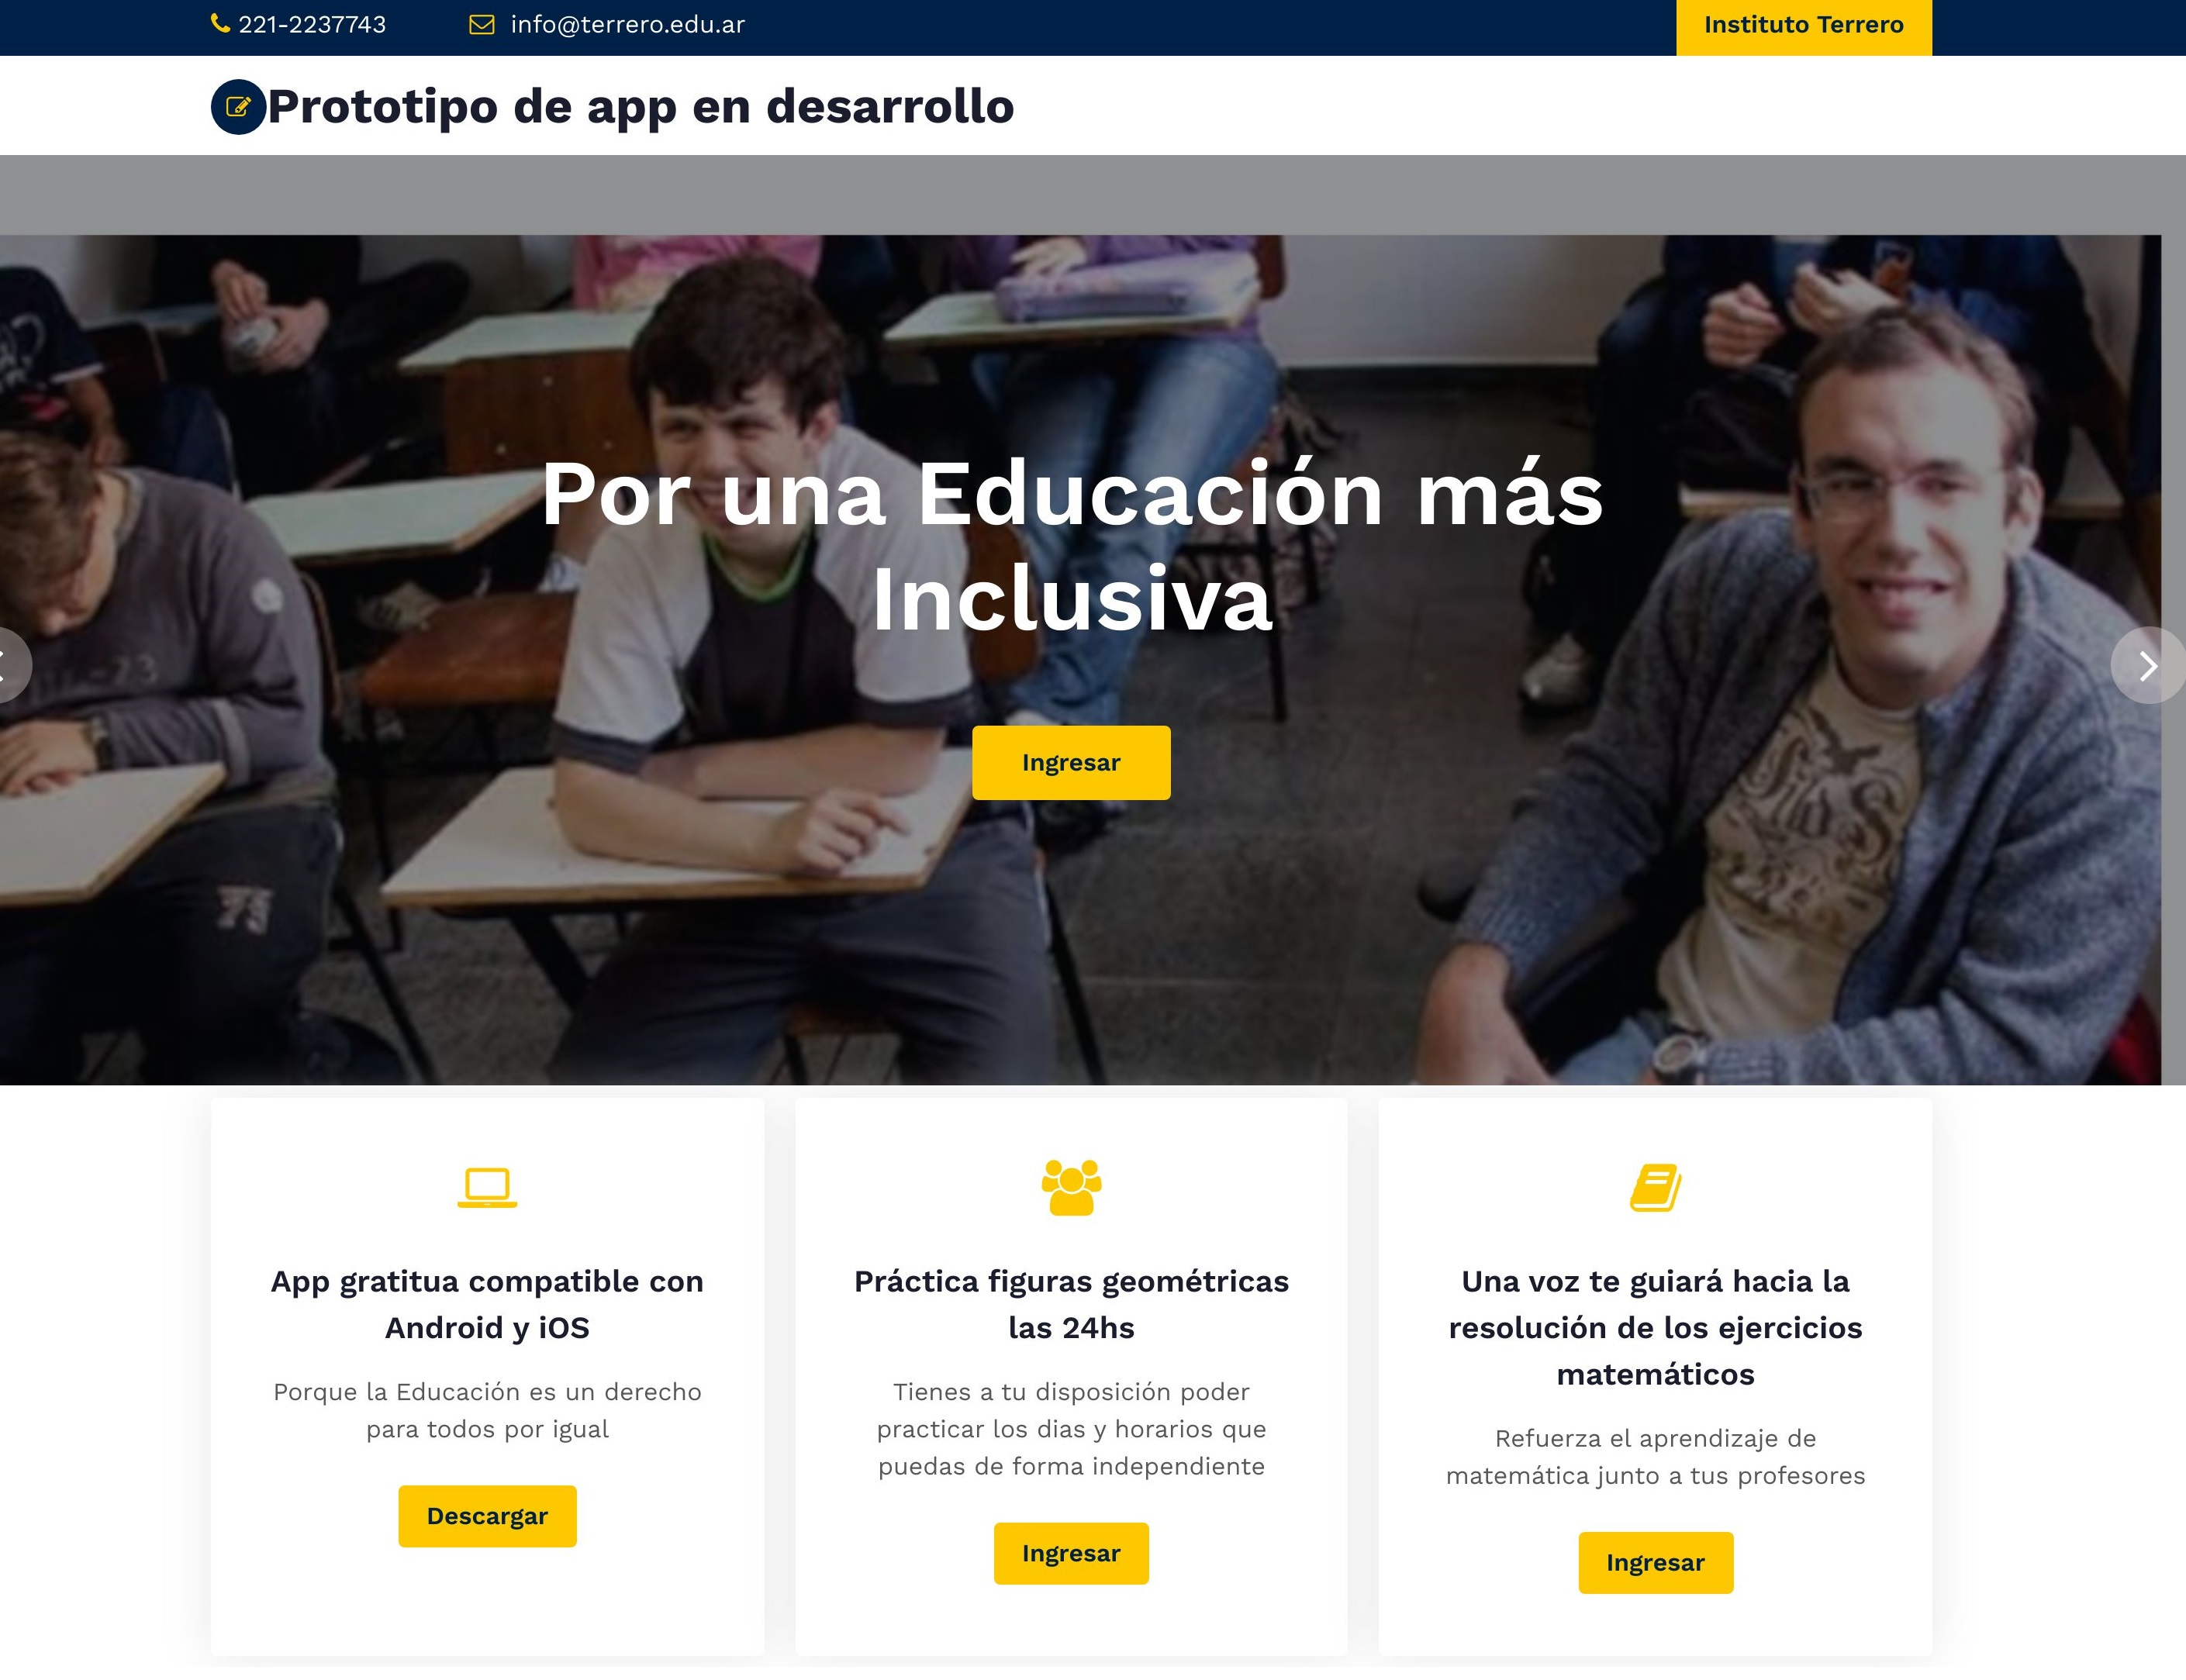
\includegraphics[width=\textwidth,height=0.5\textheight,keepaspectratio]{santimonia.org.jpg}
	\end{minipage}
	%\hspace{0.1mm}
	%\begin{minipage}[c]{0.2\textwidth}
	\begin{minipage}[c]{0.25\textwidth}
		\raggedright
	%	\vspace{-1cm}
	\begin{justify}\vspace{-0.4cm}{\changefontsizes{8.8pt}\textbf{Figura 1.} Pagina principal del prototipo accesible desde la URL:\\ \url{http://santimonia.org/accesibilidad}}\\\\
	{\changefontsizes{8.8pt}\textbf{Figura 2.} Implementación de forma muy simple del prototipo que guia por medio de voz al alumno en la realización de una figura geométrica. Accesible desde la URL \url{http://santimonia.org/accesibilidad/index19.html}}
	\end{justify}
	\end{minipage}
	\label{fig:Website}

%\vspace{1pt} % Espacio entre las imágenes
%\begin{minipage}{\textwidth}
%	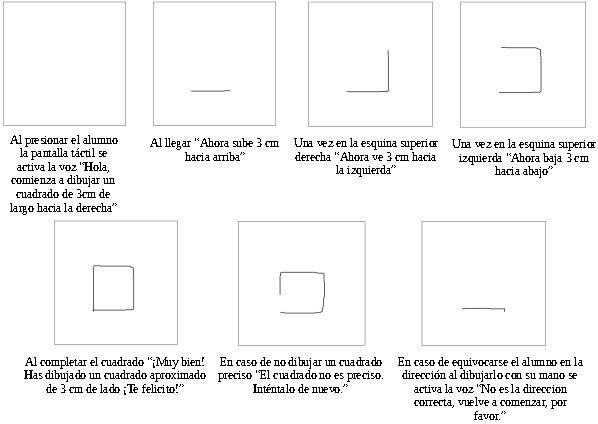
\includegraphics[width=\textwidth,height=0.4\textheight,keepaspectratio]{Guia_al_dibujar_un_cuadrado.png}
%	\label{fig:Guia}
%\end{minipage}

\end{figure}


\begin{figure}[H]
\vspace{-0.2cm}	
	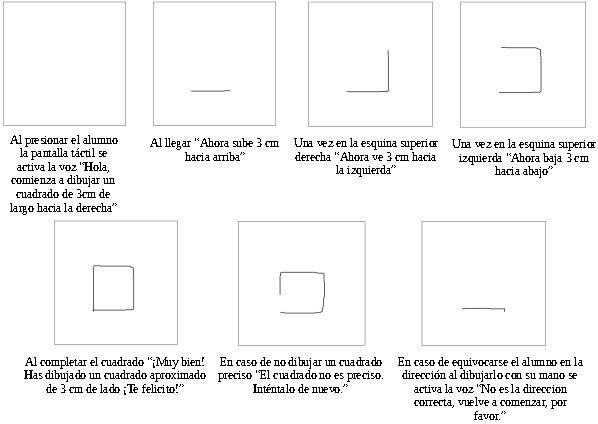
\includegraphics[width=1\textwidth,height=0.43\textheight]{Guia_al_dibujar_un_cuadrado.png}
%	\caption{Implementación de forma muy simple del prototipo que guia por medio de voz al alumno en la realización de una figura geométrica. Accesible desde la URL \url{http://santimonia.org/accesibilidad/index19.html}}
	\label{fig:Guia}
\end{figure}

\vspace{-0.49cm}
{\changefontsizes{8.8pt}
El proyecto está próximo a ser subido a GitHub que incluya la implementación que por medio de su voz (SpeechRecognition) el alumno pueda elegir la figura geométrica a dibujar, y dentro del entorno virtual, pueda obtener respuestas sobre preguntas relacionadas con las matemáticas, simulando la presencia de un tutor, al estar conectado mediante la API de Mistral AI. Se ha elegido esta empresa porque es de software libre y esta enfocada en la eficiencia energética, reduciendo el impacto ambiental contaminante que genera el procesamiento de grandes cantidades de datos (Big Data), puesto que la contaminación es unas de las causas de discapacidad-pobreza que desencadena la exclusión de las personas. La implementación en el prototipo es con Web Speech API que es compatible con la mayoría de los navegadores o browser actuales.
En un ejemplo utilizando la voz el alumno consulta al programa: “¿Qué es un cuadrado y porque tiene cuatro lados?”, esa pregunta se envía por medio de la API formando el \textit{input} que el modelo de inteligencia artificial procesa y responde utilizando el sintetizador de voz (SpeechSynthesis), las respuestas son solo a modo de ejemplo.}

%\begin{figure}[htbp]

%\begin{figure}[htbp]
%	\begin{minipage}[c]{0.60\textwidth\0.29\textwidth}
%		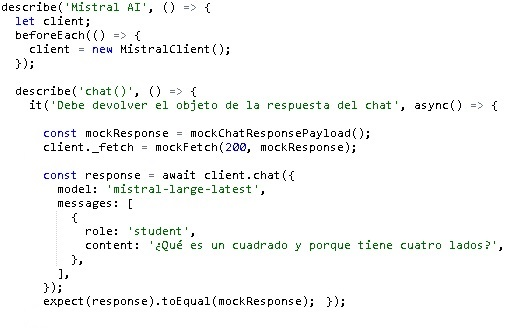
\includegraphics[width=\textwidth,height=\textheight]{ia.jpg}

		%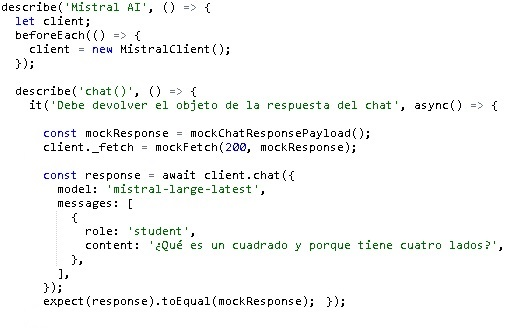
\includegraphics[width=\textwidth,height=0.29\textheight]{ia.jpg}
		%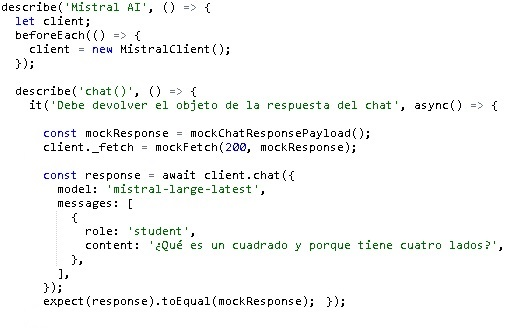
\includegraphics[width=\textwidth,height=\textheight\textheight,keepaspectratio]{ia.jpg}

%	\end{minipage}


%	%\hspace{1mm}


%	\begin{minipage}[c]{0.40\textwidth}
%		\raggedright
%		%	\vspace{-1cm} Quitado para no aumentar el margen
%		\begin{justify}
%		\begin{spacing}{0.6}{\setstretch{0.6}\changefontsizes{8.8pt}(IA):“Un cuadrado es una figura geométrica de cuatro lados iguales y cuatro ángulos rectos (de 90 grados cada uno). Tiene cuatro lados porque es un tipo específico de cuadrilátero, que es una figura con cuatro lados.”. Alumno: “¿Qué son noventa grados en un ángulo y porque el cuadrado tiene cuatro ángulos?” (AI): “Noventa grados es la medida de un ángulo recto, que es un ángulo que forma una “L”. El cuadrado tiene cuatro ángulos rectos porque es un requisito para que sus lados sean iguales y paralelos, formando una figura equilibrada.”. Alumno: “Me cuesta dibujar los cuatro lados y que me salgan iguales como puedo hacer para que me salgan bien”.
%				}
%		\end{spacing}
%		\end{justify}
%	\end{minipage}
%	\label{fig:IA}
%{\setstretch{0.6}\changefontsizes{8.8pt}\textbf{Figura 3.}Librería JS Client para la plataforma Mistral AI. Recuperado: \url{https://github.com/mistralai/client-js}}	
%\end{figure}

\begin{figure}[htbp]
	\begin{minipage}[c]{0.60\textwidth}
		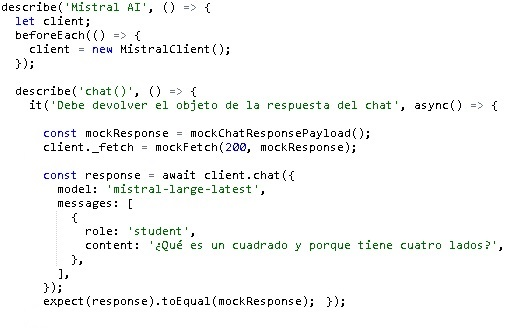
\includegraphics[width=\textwidth,height=0.285\textheight]{ia.jpg}
	\end{minipage}
	\hspace{1mm}
	\begin{minipage}[c]{0.40\textwidth}
		\raggedright
		\begin{justify}
			\begin{spacing}{0.5} % Ajusta el interlineado a 0.6 veces el interlineado normal
				\fontsize{9}{10}\selectfont % Tamaño de fuente para el texto
				(IA):\textit{“Un cuadrado es una figura geométrica de cuatro lados iguales y cuatro ángulos rectos (de 90 grados cada uno). Tiene cuatro lados porque es un tipo específico de cuadrilátero, que es una figura con cuatro lados.”}. Alumno: “¿Qué son noventa grados en un ángulo y porque el cuadrado tiene cuatro ángulos?” (AI): \textit{“Noventa grados es la medida de un ángulo recto, que es un ángulo que forma una “L”. El cuadrado tiene cuatro ángulos rectos porque es un requisito para que sus lados sean iguales y paralelos, formando una figura equilibrada.”}. Alumno: “Me cuesta dibujar los cuatro lados y que me salgan iguales como puedo hacer para que me salgan bien”.
			\end{spacing}
		\end{justify}
	\end{minipage}
	\label{fig:IA}
	\vspace{0.5em} % Espacio adicional entre la figura y el texto

	\begin{center}
			\vspace{-0.35cm}
			\changefontsizes{8.8pt}\textbf{Figura 3.} Librería JS Client para la plataforma Mistral AI. Recuperado: \url{https://github.com/mistralai/client-js}
	\end{center}
\end{figure}

\begin{figure}[h] % agrega un centimetro más de espacio
	\vspace{-0.90cm}
\end{figure}


\vspace{-1cm}

{\changefontsizes{8.8pt}
(AI): \textit{“¡Claro! Imagínate esto:
1.Dibuja una línea recta hacia el lado en la pantalla.
2.Desde el final de esa línea, dibuja una línea recta hacia arriba.
3.Desde el final de esa línea, dibuja otra línea recta hacia el lado de regreso a donde empezaste.
4.Finalmente, cierra el cuadrado dibujando una línea recta hacia abajo, de vuelta al principio.
¡Ahora tienes un cuadrado!”.}}



\section{\fontsize{12pt}{14pt}\selectfont 4 Conclusión}
% tiene que ser de 12 puntos

{\changefontsizes{8.8pt}
Es fundamental en el Siglo XXI donde nos encontramos, por la reciprocidad demostrada entre las TICs y la mejora en los aprendizajes que en todo proceso educativo, no solo relacionado con estudiantes con diversas discapacidades, estén siempre presentes. Los países más pobres económicamente son los más vulnerables, puesto que no pueden acceder al equipamiento especial o al implementar las clases de forma remota sin tener en cuenta si los estudiantes con diversas discapacidades como sucede en Ghana, un país del Continente Africano y también en países que se los llama desarrollados, como Estados Unidos, donde se evidenciaron algunos problemas donde la Pandemia de COVID19 destacó estos problemas en los aprendizajes que ya existían hace mucho tiempo, por esta y otras razones en los países consideramos pobres económicamente se omite la información de la cantidad de estudiantes con discapacidades que han abandonado sus estudios (Simeone, O., 2018)[22] , como también sucede en nuestro país, por lo que no es una cuestión solamente económica, sino política.

Como conclusión a esta introducción a la investigación de como se realizan los aprendizajes en matemáticas en niños y jóvenes con discapacidad visual sin uso de computadoras, sus dificultades en especial en las áreas de geometría y cálculo con expresiones algebraicas, y los grandes avances que han logrados diversas investigaciones que se han citado en dichos aprendizajes al incorporar el uso de las TICs en el Aula, pueda ser tomada de base para otros futuros desarrollos, entre los mismos incorporando a la IA que actualmente es muy prometedora no solo en el ámbito de la Educación, o para seguir investigando sobre este tema puesto que existe mucha biografía disponible para su análisis. El enlace del proyecto en Github es el siguiente: \url{ https://github.com/sergiooscarfauez/guidedlearning .}}

\section{\fontsize{12pt}{14pt}\selectfont 5 Agradecimientos}
% tiene que ser de 12 puntos

{\changefontsizes{8.9pt}
Agradezco a Dios y a todas las personas que han investigado junto con sus alumnos en posibles soluciones a este multidimensional problema. También quiero expresar mi gratitud a mi madre, Antonieta Sommese, quien falleció durante la pandemia, y a la Universidad Nacional de La Plata, que me ha brindado la posibilidad de realizar mis estudios, al igual que lo hizo con ella y con mi tía Francisca Benedicta Sommese, ambas egresadas de dicha Institución.
En especial, agradezco a las profesoras Lic. Díaz Lapérgola, María Ayelén y Lic. Flores, Ana Cristina por su orientación y apoyo constante a lo largo de este proyecto. Su conocimiento y experiencia han sido fundamentales para el desarrollo de esta investigación, la cual forma parte del trabajo realizado para el Portfolio final de las materias Perspectiva Filosófico Pedagógico II y Perspectiva Pedagógico Didáctica II, y al Instituto Superior del Profesorado J. N. Terrero, de las carreras de Profesorado en Ciencia Sagrada y Profesorado en Filosofía.}

\section{\fontsize{12pt}{14pt}\selectfont 6 Referencias}
% tiene que ser de 12 puntos

\begin{enumerate}[noitemsep, topsep=0pt, parsep=0pt, partopsep=0pt]
	{\changefontsizes{8.9pt}
		\setlength{\itemsep}{0pt}
		\item Agencia Nacional de Discapacidad, ``8 de cada 10 personas con discapacidad no tienen trabajo en Argentina,'' \emph{Página12}, 2022. URL  \url{https://www.pagina12.com.ar/464426-8-de-cada-10-personas-con-discapacidad-no-tienen-trabajo-en-argentin}.
		\item J. Bellina Yrigoyen, ``Discapacidad, mercado de trabajo y pobreza en Argentina,'' \emph{Dialnet}, 2013. URL  \url{https://dialnet.unirioja.es/descarga/articulo/4234635.pdf}.
		\item \emph{La Nación}, ``Discapacidad visual. Entregarán dispositivos que pasan texto a voz a estudiantes secundarios,'' 2023. URL  https://www.lanacion.com.ar/sociedad/discapacidad-visual-entregaran-dispositivos-que-pasan-texto-a-voz-a-estudiantes-secundarios-nid11022023/.
		\item Centro de Implementación de Políticas Públicas para la Equidad y el Crecimiento (CIPPEC), ``El impacto de la pandemia en la educación secundaria en Argentina y América Latina,'' 2023. URL  \url{https://www.cippec.org/proyecto/el-impacto-de-la-pandemia-en-la-educacion-secundaria/}.
		\item Dirección Nacional de Evaluación, Información y Estadística Educativa, \emph{Informe Nacional de Indicadores Educativos: situación y evolución del derecho a la educación en Argentina}, 1a ed., Ciudad Autónoma de Buenos Aires: Ministerio de Educación de la Nación, 2022. ISBN: 978-950-00-1583-7. URL  \url{https://www.argentina.gob.ar/sites/default/files/informe_nacional_indicadores_educativos_2021_2_1.pdf}.
		\item S. Gajardo Alveal y O. M. Rojas Zavala, ``Aprendizaje de matemática en estudiantes en situación de discapacidad visual que acceden a la educación secundaria. Un estudio de caso,'' Universidad de Concepción, 2017. URL  \url{http://repositorio.udec.cl/bitstream/11594/2510/4/Alveal Rojas.pdf}.
		\item Organización Mundial de la Salud, \emph{Informe mundial sobre la visión}, Ginebra: OMS, 2020. URL  \url{https://apps.who.int/iris/bitstream/handle/10665/331423/9789240000346-spa.pdf}.
		\item M. Gallegos Navas, \emph{La inclusión de las TIC en la educación de personas con discapacidad. Relatos de experiencias}, Quito: Universidad Politécnica Salesiana, 2018. ISBN: 978-9978-10-331-9. URL  \url{https://dspace.ups.edu.ec/bitstream/123456789/17078/1/La%20inclusio%CC%81n%20de%20las%20TIC%20en%20la%20educacion%20de%20personas%20con%20discapacidad.pdf}.
		\item Consejería de Educación, Dirección General de Participación e Innovación Educativa, Junta de Andalucía, \emph{Manual de atención al alumnado con necesidades específicas de apoyo educativo derivadas de discapacidad visual y sordoceguera}, ISBN: 978-84-691-8128-7, 2008. URL  \url{https://sid-inico.usal.es/idocs/F8/FDO23841/apoyo_educativo_visual_sordoceguera.pdf}.
		\item M. A. Cinquegrani, \emph{Entre la resistencia, el amor y la esperanza. Familias, discapacidad y educación}, Buenos Aires: Editorial Biblos, 2022. ISBN: 978-987814-024-7.
		\item C. Fernández, ``La situación del derecho a la educación inclusiva en América Latina,'' en \emph{Ciclo de Webinarios sobre Educación Inclusiva}, Organización de los Estados Americanos (OEA)-Red Regional por la Educación Inclusiva de Latinoamérica (RREI), 2018.
		\item \emph{Ley de Educación Nacional 26.206}, República Argentina, 2006.
		\item F. J. Soto Pérez, ``Promoviendo el uso de tecnologías inclusivas en contextos educativos diversos,'' \emph{Entera 2.0. Revista Digital}, vol. 1, pp. 14-22, 2013. URL  \url{https://www.ciberespiral.org/enterados/wp-content/uploads/2013/09/Soto-TICInclusivas.pdf}.
		\item B. A. Rueda Díaz, ``Implementación de un dispositivo de enlace entre docentes y estudiantes con discapacidad visual en el área de matemáticas,'' \emph{EDEDVAM}, Universidad Pedagógica Nacional, Universidad Militar Nueva Granada, 2020.
		\item E. A. Gutiérrez Molano y O. Guataquira Quevedo, ``Estrategias de aprendizaje de matemáticas en estudiantes con ceguera o baja visión,'' Universidad Nacional Abierta y a Distancia (UNAD), Escuela Ciencias de la Educación (ECEDU), 2017. URL  \url{https://repository.unad.edu.co/handle/10596/12082}.
		\item ONG Educo, ``Aplicaciones de inteligencia artificial (IA) en la educación,'' 2023. URL  \url{https://www.educo.org/blog/aplicaciones-de-ia-en-la-educacion}.
		\item A. R. Sadykova y I. V. Levchenko, ``La inteligencia artificial como componente del contenido innovador de la educación general: análisis de la experiencia mundial y perspectivas nacionales,'' \emph{Revista de la Universidad Rusa de la Amistad de los Pueblos}, 2020.
		\item ``Inteligencia Artificial en la Educación,'' \emph{Boletín pedagógico de Sebastopol}, 2020.
		\item K. Singh, ``La educación es un bien público y una obligación moral,'' \emph{Semana de Acción Mundial para la Educación}, UNESCO, 2016. URL  https://www.unesco.org/es/articles/semana-de-accion-mundial-para-la-educacion-laeducacion-es-un-bien-publico-y-una-obligacion-moral.
		\item F. Contreras y M. Alejo, ``Educación: base del desarrollo humano,'' \emph{Revista Digital Postgrado}, vol. 8, no. 2, e177, 2019. URL  \url{http://portal.amelica.org/ameli/jatsRepo/101/101676008/html/index.htm}.
		\item M. L. Iovanovich, ``El pensamiento de Paulo Freire: sus contribuciones para la educación,'' CLACSO, Consejo Latinoamericano de Ciencias Sociales, 2003. URL  \url{https://biblioteca.clacso.edu.ar/clacso/formacionvirtual/20100720092748/19iovanovich.pdf}.
		\item O. Simeone, ``A very brief introduction to Machine Learning with applications to Communication Systems,'' \emph{Institute of Electrical and Electronics Engineers (IEEE)}, 2018. URL  \url{https://ieeexplore.ieee.org/document/8542764}.
	}
\end{enumerate}


%\begin{enumerate}
%	\def\labelenumi{\arabic{enumi}.}
%	\item
%	Author, F.: Article title. Journal 2(5), 99--110 (2016).
%	\item
%	Author, F., Author, S.: Title of a proceedings paper. In: Editor, F.,
%	Editor, S. (eds.) CONFERENCE~2016, LNCS, vol. 9999, pp.~1--13.
%	Springer, Heidelberg (2016).
%	\item
%	Author, F., Author, S., Author, T.: Book title. 2nd edn. Publisher,
%	Location (1999).
%	\item
%	Author, F.: Contribution title. In: 9th International Proceedings on
%	Proceedings, pp. 1--2. Publisher, Location (2010).
%	\item
%	LNCS Homepage, \url{http://www.springer.com/lncs}, last accessed
%	2016/11/21.
%\end{enumerate}


%Subsequent paragraphs, however, are indented.

%\subsubsection{\texorpdfstring{\textbf{Sample Heading (Third Level).}
%Only two levels of headings should be numbered. Lower level headings
%remain unnumbered; they are formatted as run-in
%headings.}{Sample Heading (Third Level). Only two levels of headings should be numbered. Lower level headings remain unnumbered; they are formatted as run-in headings.}}\label{sample-heading-third-level.-only-two-levels-of-headings-should-be-numbered.-lower-level-headings-remain-unnumbered-they-are-formatted-as-run-in-headings.}

%\paragraph{\texorpdfstring{\emph{Sample Heading (Forth Level).} The
%contribution should contain no more than four levels of headings. The
%following Table 1 gives a summary of all heading
%levels.}{Sample Heading (Forth Level). The contribution should contain no more than four levels of headings. The following Table 1 gives a summary of all heading levels.}}\label{sample-heading-forth-level.-the-contribution-should-contain-no-more-than-four-levels-of-headings.-the-following-table-1-gives-a-summary-of-all-heading-levels.}

%\protect\hypertarget{_Ref467509391}{}{}\textbf{Table 1.} Table captions
%should be placed above the tables.

%\begin{longtable}[]{@{}lll@{}}
%\toprule
%Heading level & Example & Font size and style\tabularnewline
%\midrule
%\endhead
%Title (centered) & \textbf{Lecture Notes} & 14 point,
%bold\tabularnewline
%1\textsuperscript{st}-level heading & \textbf{1 Introduction} & 12
%point, bold\tabularnewline
%2\textsuperscript{nd}-level heading & \textbf{2.1 Printing Area} & 10
%point, bold\tabularnewline
%3\textsuperscript{rd}-level heading & \textbf{Run-in Heading in Bold.}
%Text follows & 10 point, bold\tabularnewline
%4\textsuperscript{th}-level heading & \emph{Lowest Level Heading.} Text
%follows & 10 point, italic\tabularnewline
%\bottomrule
%\end{longtable}

%Displayed equations are centered and set on a separate line.

%\emph{x} + \emph{y} = \emph{z}
%(1\protect\hypertarget{_Ref467511674}{}{})

%Please try to avoid rasterized images for line-art diagrams and schemas.
%Whenever possible, use vector graphics instead (see Fig. 1).

%\protect\hypertarget{_Ref467515387}{}{}\textbf{Fig. 1.} A figure caption
%is always placed below the illustration. Short captions are centered,
%while long ones are justified. The macro button chooses the correct
%format automatically.

%For citations of references, we prefer the use of square brackets and
%consecutive numbers. Citations using labels or the author/year
%convention are also acceptable. The following bibliography provides a
%sample reference list with entries for journal articles {[}1{]}, an LNCS
%chapter {[}2{]}, a book {[}3{]}, proceedings without editors {[}4{]}, as
%well as a URL {[}5{]}.

%References

%\begin{enumerate}
%\def\labelenumi{\arabic{enumi}.}
%\item
%  Author, F.: Article title. Journal 2(5), 99--110 (2016).
%\item
%  Author, F., Author, S.: Title of a proceedings paper. In: Editor, F.,
%  Editor, S. (eds.) CONFERENCE~2016, LNCS, vol. 9999, pp.~1--13.
%  Springer, Heidelberg (2016).
%\item
%  Author, F., Author, S., Author, T.: Book title. 2nd edn. Publisher,
%  Location (1999).
%\item
%  Author, F.: Contribution title. In: 9th International Proceedings on
%  Proceedings, pp. 1--2. Publisher, Location (2010).
%\item
%  LNCS Homepage, \url{http://www.springer.com/lncs}, last accessed
%  2016/11/21.
%\end{enumerate}

\end{document}
